\documentclass[conference]{IEEEtran}
\usepackage{amsmath,amssymb,amsfonts}
\usepackage{algorithmic}
\usepackage{graphicx}
\usepackage{textcomp}
\usepackage{xcolor}
\usepackage[style=ieee]{biblatex}
\addbibresource{refs.bib}

\begin{document}
\title{Characterizing hippocampal replay using hybrid point process state space models}

\author{\IEEEauthorblockN{1\textsuperscript{st} Eric L. Denovellis}
\IEEEauthorblockA{\textit{Dept. of Physiology} \\
\textit{Univ. of California, San Francisco}\\
San Francisco, CA, USA \\
https://orcid.org/0000-0003-4606-087X}
\and
\IEEEauthorblockN{2\textsuperscript{nd} Loren M. Frank}
\IEEEauthorblockA{\textit{Dept. of Physiology} \\
\textit{Univ. of California, San Francisco}\\
San Francisco, CA, USA \\
loren@phy.ucsf.edu}
\and
\IEEEauthorblockN{3\textsuperscript{rd} Uri T. Eden}
\IEEEauthorblockA{\textit{Dept. of Mathematics and Statistics} \\
\textit{Boston University}\\
Boston, MA, USA \\
tzvi@bu.edu}

}

\maketitle

\begin{abstract}
In the hippocampus, replay sequences are temporally compressed patterns of cell activity that resemble patterns that occur when the animal is moving through the environment. Because replay sequences typically occur when the animal is at rest, replay is hypothesized to be part of an internal cognitive process that enables the retrieval of past spatial memories and the planning of future movement. Traditionally, replay sequences have been discovered by looking for sharp wave ripples---high frequency oscillations that occur in association with replay---and then looking for spatially continuous patterns of cell activity; however, it has become clear that this does not fully depict the complexity of replay sequences. Replay sequences do not always co-occur with sharp wave ripples, have more complex dynamics than spatially continuous movement, have different temporal ordering than during movement, and change based on task. In this work, we introduce a hybrid state space framework to describe the richness of replay sequences. We show how defining discrete latent states associated with continuous latent dynamics and point process observations allows us to identify when replay sequences occur, categorize the type of sequence based on their proscribed continuous dynamics, and decode the spatial trajectory corresponding to the replay sequence.

\end{abstract}

\begin{IEEEkeywords}
State-space methods, Hippocampus, Replay, Switching liner dynamical systems, Point process
\end{IEEEkeywords}

\section{Introduction}
A central question in neuroscience is how patterns of neuronal activity in the brain correspond to the formation and use of memories. But understanding memory is challenging because it is a unobserved, internal state of mind which does not necessarily correspond to the animal’s current behavior and the corresponding neuronal activity patterns in the brain are noisy, high-dimensional, and can rapidly change on short timescales. As a result, neuroscientists need statistical methods that are flexible enough to capture the dynamically changing state of the brain, but remain interpretable enough to understand what those states are.

An example of this challenge is hippocampal replay. In the hippocampus---a brain area known for its role in memory and early learning---neurons selectively respond based on position in the environment \cite{OKeefehippocampusspatialmap1971}, the population pattern of spiking activity reflecting the trajectory of the animal. When the animal is asleep or immobile, these activity patterns reappear, but on a shorter timescale \cite{WilsonReactivationhippocampalensemble1994, NadasdyReplayTimeCompression1999}. Because of the similarity of the patterns to previous behavior and the compressed nature of the activity, the “replayed” activity patterns are thought to correspond to animal's memory of previously moving through the environment. But recent work has shown that the replayed pattern of activity can be quite diverse. For example, replay activity patterns can occur in the reverse order to when it occurred during behavior \cite{FosterReversereplaybehavioural2006, DibaForwardreversehippocampal2007}, can correspond to different environments \cite{KarlssonAwakereplayremote2009}, and can have finer timescale dynamics which possibly relate to the underlying computations performed in the brain \cite{PfeifferAutoassociativedynamicsgeneration2015}. Therefore, it is important for neuroscientists to have methods that are flexible enough to capture these changes in dynamics while still being able interpret them.

Point process state space models have been successful solution to categorizing different types of replay via their dynamics \cite{DengRapidclassificationhippocampal2016, EdenCharacterizingComplexMultiScale2018}. Previously, we have used state space models with parallel point process filters to classify task dependent trajectories in a real-time setting \cite{DengRapidclassificationhippocampal2016}. Here we extend that model to a general state-space state space framework for characterizing hippocampal replay. We show how this framework can: (1) allow for switching between discrete states by adding in a model of the discrete dynamics (2) used in offline analysis by adding an acausal smoother, and (3) be flexible and interpretable by associating with discrete states with a particular continuous dynamic, initial condition and likelihood. We illustrate this more concretely by showing two examples of how this framework can be used to characterize features of replay.

\section{Methods}
\subsection{Problem Definition}
We want to model how spiking patterns from neurons correspond to features of replay and how those features evolve over time. Let $I_{k}$ be a discrete latent state variable that corresponds to a set of features of replay that are of interest and $x_{k}$ be a continuous latent state variable that corresponds to the position represented by the population of neurons at time $t_{k}$. For example, the discrete latent variable could be an indicator function that distinguishes between task dependent forward and reverse order replays as in \cite{DengRapidclassificationhippocampal2016}, an indicator function that distinguishes between replay trajectories on the current spatial environment versus a previously experienced spatial environment, or an indicator function that distinguishes between replays that move toward the animal's location versus away from the animal's position. In each of these scenarios, $x_{k}$ is a representation for how the position represented by the neurons coevolves with each of these different discrete categories.

We want to estimate how the latent variables change depending on the observed data. For each neuron, we observe a collection of spike times---times when an action potential occurs. Let $\Delta N_{k}$ be the number of spikes between the time interval $t_{k}$ and $t_{k-1}$ for a single neuron. Assuming we have a collection of $C$ neurons and we observe spiking observations from these neurons from time $1$ up to time $T$, the problem is then to infer the joint posterior probability of the latent variables given the spiking data $p(x_{k}, I_{k} \mid \Delta N_{1:T}^{(1:C)})$. In order to do this, we will first estimate the causal filter posterior $p(x_{k}, I_{k} \mid \Delta N_{1:k}^{(1:C)})$, which only takes into account the past observations, and then use this quantity to estimate the acausal smoother density $p(x_{k}, I_{k} \mid \Delta N_{1:T}^{(1:C)})$, which takes into account both past and future observations.

\subsection{Causal Filter}
We can use Bayes theorem to define the posterior $p(x_{k}, I_{k} \mid \Delta N_{1:k}^{(1:C)})$ in terms of the likelihood of the spiking data $p(\Delta N_{k}^{(1:C)} \mid x_{k}, I_{k})$ and a prior $p(x_{k}, I_{k} \mid \Delta N_{1:k-1}^{(1:C)})$:
\begin{multline}
p(x_{k}, I_{k} \mid \Delta N_{1:k}^{(1:C)}) \propto \\
p(\Delta N_{k}^{(1:C)}  \mid x_{k}, I_{k}) p(x_{k}, I_{k} \mid \Delta N_{1:k-1}^{(1:C)}) 
\end{multline}

If we assume the dynamics of the latent variables can be described by a Markov process, we can then use the \textit{Chapman-Kolmogorov equation} to recursively define the prior $p(x_{k}, I_{k} \mid \Delta N_{1:k-1}^{(1:C)})$ in terms of previous time step's posterior, yielding the one-step prediction density:
\begin{multline}
p(x_{k}, I_{k} \mid \Delta N_{1:k-1}^{(1:C)}) = \\
\sum_{I_{k-1}} \int p(x_{k} \mid x_{k-1}, I_{k}, I_{k-1}) Pr(I_{k} \mid I_{k-1}) \\
\times p(x_{k-1}, I_{k-1} \mid \Delta N_{1:k-1}^{(1:C)}) dx_{k-1}
\end{multline}

The one-step prediction density consists of three main terms: the continuous state transition $p(x_{k} \mid x_{k-1}, I_{k}, I_{k-1})$, the discrete state transition $Pr(I_{k} \mid I_{k-1})$, and the previous time step's posterior $p(x_{k-1}, I_{k-1} \mid \Delta N_{1:k-1}^{(1:C)})$. The discrete state transition dictates the probability of remaining in a discrete state or switching to one of the other discrete states. The continuous state transition dictates how the latent position evolves. Note that the continuous state transition depends on the current discrete state $I_{k}$, the past discrete state $I_{k-1}$ and the previous latent position $x_{k-1}$. This enforces the latent dynamics of the model, whereby continuous states depend on the discrete states.

When we combine the one-step prediction density with the data likelihood we have:
\begin{multline}
p(x_{k}, I_{k} \mid \Delta N_{1:k}^{(1:C)}) \propto \\
p(\Delta N_{k}^{(1:C)}  \mid x_{k}, I_{k}) \sum_{I_{k-1}} \int p(x_{k} \mid x_{k-1}, I_{k}, I_{k-1}) \\
\times Pr(I_{k} \mid I_{k-1}) p(x_{k-1}, I_{k-1} \mid \Delta N_{1:k-1}^{(1:C)}, dx_{k-1})
\end{multline}
as the final filter.

Lastly, we have to define the likelihood $p(\Delta N_{k}^{(1:C)} \mid x_{k}, I_{k})$. We model the spiking observations from each cell as a point process that is conditionally independent given the continuous and discrete latent processes. Point processes are completely described by their conditional intensity function $\lambda(t)$, which is the instantaneous probability of observing a spike at time $t$.

\begin{equation}
    \lambda(t \mid H_{t}) = \lim_{\Delta t \rightarrow{0}} \frac{Pr(N(t + \Delta t) - N(t) = 1 \mid x_{t}, I_{t})}{\Delta t}
\end{equation}


\begin{multline}
    p(\Delta N_{k}^{(1:C)} \mid x_{k}, I_{k}) = \prod^{C}_{i=1} ((\lambda_{i}(t_{k} \mid x_{k}, I_{k})\Delta_{k})^{N_{t_{k}}^{i}} \\
    \times \exp(-\lambda_{i}(t_{k} \mid x_{k}, I_{k})\Delta_{k})
\end{multline}

\subsection{Acausal Smoother}
Assuming the causal filter $p(x_{k}, I_{k} \mid \Delta N_{1:k}^{(1:C)})$ has been computed for all $k = 0, ..., T$, we want to compute $p(x_{k}, I_{k} \mid \Delta N_{1:T}^{(1:C)})$ for all $k < T$. This is known as the fixed-interval smoother and at any given time, it takes into account spiking observations in the past and future (except at 0 and time $T$). Similar to the filter posterior, this can also be expanded into a recursive formula that now uses the future smoother posterior $p(x_{k+1}, I_{k+1} \mid \Delta N_{1:T}^{(1:C)})$ and filter posterior $p(x_{k}, I_{k} \mid \Delta N_{1:k}^{(1:C)})$ at time step $k$.
\begin{multline}
p(x_{k}, I_{k} \mid \Delta N_{1:T}^{(1:C)}) = \\
p(x_{k}, I_{k} \mid \Delta N_{1:k}^{(1:C)}) \\
\times \sum_{I_{k+1}} \int \frac{p(x_{k+1} \mid x_{k}, I_{k+1}, I_{k}) Pr(I_{k+1} \mid I_{k})}{p(x_{k+1}, I_{k+1} \mid \Delta N_{1:k}^{(1:C)})} \\
\times p(x_{k+1}, I_{k+1} \mid \Delta N_{1:T}^{(1:C)}) dx_{k+1}
\end{multline}.

The continuous state transition $p(x_{k+1} \mid x_{k}, I_{k+1}, I_{k})$ and discrete state transition $Pr(I_{k+1} \mid I_{k})$ can be the same as used for the filter. Finally, the denominator in the integral can be expanded in terms of the state transitions and filter posterior.
\begin{multline}
p(x_{k+1}, I_{k+1} \mid \Delta N_{1:k}^{(1:C)}) = \\
\sum_{I_{k}} \int p(x_{k+1} \mid x_{k}, I_{k+1}, I_{k}) Pr(I_{k+1} \mid I_{k}) \\
\times p(x_{k}, I_{k} \mid \Delta N_{1:k}^{(1:C)}) dx_{k}
\end{multline}
This is just the one-step prediction density for the current time step's filter posterior.

\subsection{Estimation}
\section{Results}
\subsection{Example 1}
\begin{figure}[ht]
\centerline{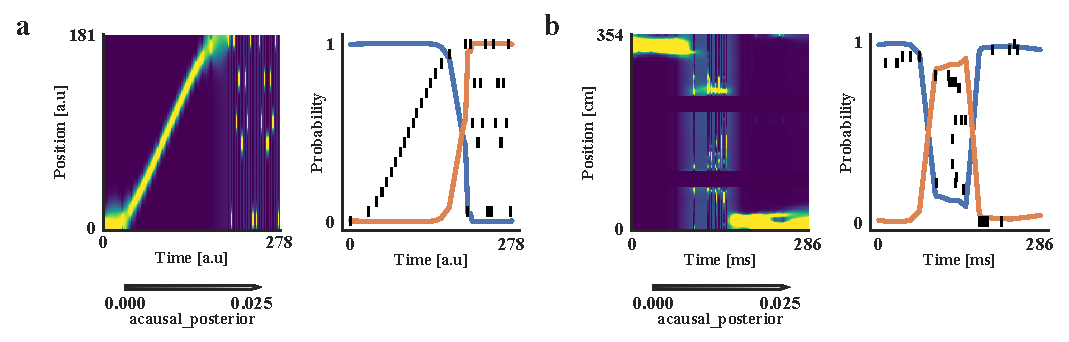
\includegraphics{fig1.pdf}}
\caption{Example of a figure caption.}
\label{fig}
\end{figure}

\subsection{Example 2}
\section{Conclusion}
In this work, we have developed a point process state-space framework for understanding hippocampal replay that associates discrete latent states with continuous latent dynamics and allows for switching between the discrete states. We showed this framework is flexible: it can be deployed to characterize whether a replay represents spatially continuous trajectories or spatially discontinuous trajectories or it can be deployed to characterize local and non-local patterns of activity. Although we have only shown two examples of this framework, one could imagine combining the examples into one model---specifying that only during non-local states do we care about whether the trajectory is spatially continuous or not for example---or specifying more complicated conditions. All one has to specify is the initial condition, the likelihood, and state transition dynamic associated with each discrete state. The discrete state is then immediately interpretable in terms of the model.

This combination of interpretability and flexibility makes the framework is extremely powerful. By formulating what needs to be characterized mathematically, neuroscientists are forced to explicitly formulate their mental model of the replay characteristics of interest. This model can then be evaluated based on the data, criticized if the model assumptions are not adequate and improved into a better model. This iterative model building approach should be particularly powerful with respect to the hippocampus, where there are well-established features of the data and corresponding theories about the functioning of the hippocampus. The richness of data and theory allows neuroscientists to take advantage of both the flexibility of the framework and the specificity that it allows.


\section*{Acknowledgments}
\printbibliography
\end{document}



